\chapter{针对硬件加速层的 GPU 地址随机化逆向分析框架}
\section{引言}
近年来，由于 AI 技术的快速崛起，图形处理单元 （Graphics Processing Unit, GPU）作为机器学习模型训练所需的核心硬件，已经在 AI 领域发挥了举足轻重的作用。这得益于其架构上有数千个更小、更高效的并行运算单元，使其能够保持极高的吞吐量，从而快速地训练复杂神经网络和大模型参数。在所有的 GPU 中，英伟达 GPU 凭借其强大的性能和良好的软件生态系统，一直保持其在独立 GPU 市场的领先统治地位，据现有报道显示，英伟达 GPU 在 2025 年已经占到了 93\% 的市场份额~\cite{nv_gpu_share}。然而随着英伟达 GPU 的越来越普及，其作为硬件加速层的核心组件，其在供应链层面的安全性也愈发变得重要。

为了保障自身 GPU 的安全性，英伟达在其驱动，固件以及用户态库三个供应链层面做了大量的安全机制，其中最为重要的一项是为了保护其 GPU 上内存布局而设置的地址空间布局随机化技术（Address Space Layout Randomization, ASLR），该举措能够使得英伟达统一计算设备架构（Compute Unified Device Architecture, CUDA）代码在运行时随机化关键组件使用的内存地址，从而使攻击者更难猜测和定位到关键信息地址后实行内存损坏攻击。现有大量工作针对 CPU 侧的 ASLR 研究，包括探索 ASLR 随机化熵的不足和各种加强地址随机化的举措~\cite{binosi2024illusion,diaz2021address,tagbleed2020}。但是对于 GPU 上 ASLR 的实现细节和安全影响目前仍然存在很大的未知区域。Zhang 等人和 Mittal 等人最早开始研究 GPU 侧内存布局并总结出 GPU 上并未实现 ASLR 的错误结论~\cite{zhang2022lak,mittal2018survey}。随后 Hoover 等人 和 Cismaru 等人通过实验首次正式了英伟达 GPU 上存在 ASLR 机制，然而他们并未深入分析~\cite{hoover2022analysis,cismaru2023study}。Park 等人进一步发现，GPU 仅对代码段和数据段进行随机化，未对 CUDA GPU 运行时库进行随机化~\cite{park2020mind}。因此，目前针对 GPU ASLR 的主要研究都集中于是否存在随机化以及 GPU 内存相关操作分析上，目前仍然缺乏对英伟达 GPU 上 ASLR 实现机制的全面审查。

为了填补这一研究空白，本研究提出了一套针对硬件加速层的 GPU 地址随机化逆向分析框架，用以解决英伟达生态黑盒不开源的难题。该框架不仅重建 GPU 侧的内存布局，还提出了 \code{FlagProb} 技术用于深入分析GPU内存布局的 和 \code{AnchorTrace} 技术用于高效搜集 GPU 上随机化地址。这些技术不仅使 GPU 内存布局和 ASLR 进行全面分析成为可能，也揭示了 NVIDIA ASLR 实现中以前未知的弱点。总的来说，本章节主要包括了以下四个方面的创新性工作：

首先，本研究首次对英伟达 GPU 上的 ASLR 具体实现进行了系统性地分析，不仅分析了 GPU 上的内存布局及其每块内存的完整语义，更逆向出了泄漏 GPU 地址的专用内存，用以帮助搜集 GPU 侧随机化地址，从而帮助随机化分析。

在技术方面，由于英伟达 GPU 黑盒特性，GPU 上内存块语义是完全未知的，并且大量的内存区域对用户是隐藏的，导致无法通过常规调试工具进行访问或者观察，因此必须依靠逆向工程来揭示这些内存块的语义。其次在 CPU 上分析 ALSR 的技术往往在 GPU 上不适用，例如传统的 \code{printf} 或者 \code{printk} 打印地址的方式并无法打印出隐藏段的地址；传统利用页表搜集随机化地址的方式由于每次执行都需要转储大量 GPU 物理内存后进行解析导致存在不可容忍的开销。为了应对这些挑战，本研究提出了两项新型技术，用于深入分析 GPU 内存布局的 \code{FlagProb} 技术和用于高效收集 ASLR 地址的\code{AnchorTrace} 技术，并将这两项技术整合为一项针对 AI 系统的硬件加速层的 GPU ASLR 逆向分析框架。

其次在威胁评估方面，本研究发现了大量 GPU 上的内存布局缺陷。在 GPU 内存布局上，本研究发现所有 CUDA 进程共享两块大型 GPU 内存区域，还将一个 CPU 内核空间页映射到了具有用户权限的 GPU 进程内存布局中。此外，CPU 和 GPU 都将一些各自设备上的物理内存页映射到了各自的虚拟地址空间中，但权限不同：GPU 具有读写执行访问权限，而 CPU 被限制为读写权限。这些 CUDA 进程之间这些共享的内存区域为隐蔽信道攻击提供了便利，而权限不同的 GPU 和 CPU 内存共享使得潜在的跨处理器攻击成为可能——例如从 CPU 注入 GPU 可执行代码，或在 GPU 上构造恶意数据以破坏 CPU。本研究还观察到，GPU 上的堆内存区域并未完全随机化，而即使随机化的内存区域，如代码段和 CUDA 库段，都使用相同的 ASLR 偏移量进行随机化，这种粗粒度的随机化机制削弱了 GPU ASLR 的有效性。

最后在新型攻击方面，本研究发现 CPU 上的 \code{glibc} 段内存地址和 GPU 上部分区域的随机化地址存在特定联系，其二者地址的偏移量的随机化熵仅仅只有 7 位的变化，这种 ASLR 偏移相关性允许攻击者从 GPU 推断出 CPU 侧的随机化地址。利用该弱点本研究提出了一项新型的跨设备攻击，利用简单的栈越界读取来泄漏 GPU ASLR 地址，然后利用相关联的偏移量推断出 CPU 的 ASLR 偏移量。这表明 GPU ASLR 不仅自身的安全性有限，而且还进一步破坏了 CPU 上的 ASLR 保护机制。

\subsection{背景知识}

\begin{figure}[t]
    \centering
    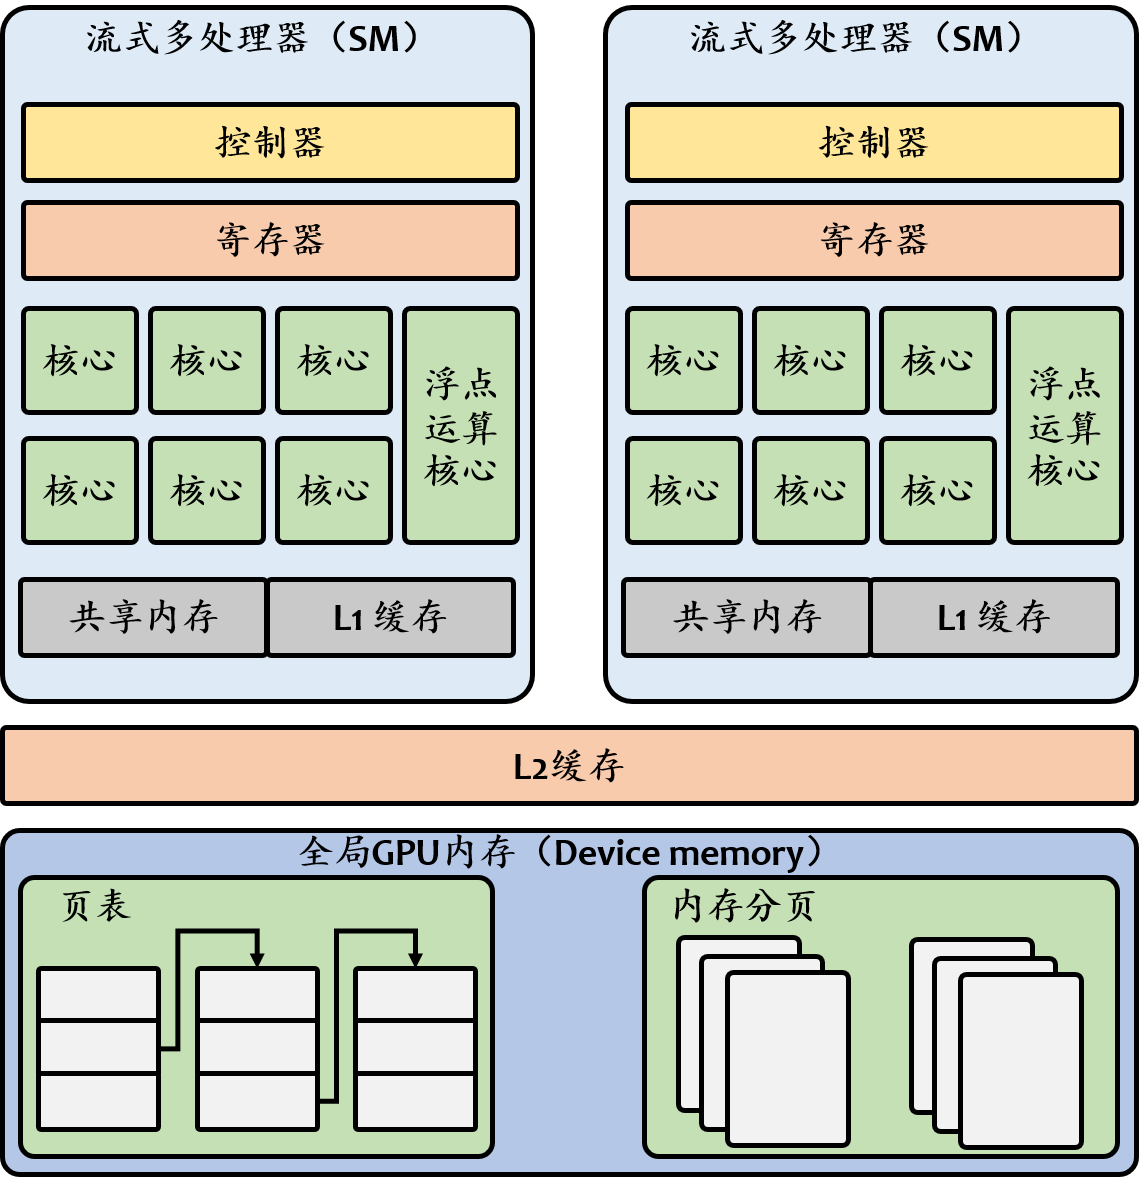
\includegraphics[width=0.7\linewidth]{figure/GPU 硬件架构.png}
    \caption{\label{fig:gpu_architecture}GPU硬件架构图}
\end{figure}

\subsubsection{英伟达 GPU 硬件架构}
如图~\ref{fig:gpu_architecture}描述了 GPU 在硬件上的架构实现。和 CPU 不同的是，GPU上的核心叫流式多处理器（Streaming Multiprocessors, SM），每一个 SM 包含了多个整型运算核心和浮点运算核心，这些运算核心可以以单指令多数据流的方式执行一组并行线程，这些并行线程通常被称为一个 warp（通常是 32 个线程），也是 GPU 调度的最小单位。现代 GPU 通常包含几十甚至上百个 SM，因此一个 GPU 往往可以同时运行上千个线程。除此之外，每个 SM 都包含自己特有的通用寄存器，用以支持多个线程的并行运行，这些通用寄存器会在线程运行时进行动态分配，并且用以存储运算临时数据。

此外，GPU 为了运算加速，在硬件上还提供了多级缓存机制，在每一个 SM 内部存在一个一级缓存，用于不同线程之间共享，而所有的 SM 共享一个二级缓存，在内存最底层是全局的设备内存，也就是人们常说的显存。值得注意的是，CPU 和 GPU 的内存系统是相互独立的，和 CPU 包含内存运算单元执行页表翻译类似，GPU 也包含了 GPU 内存运算单元（GPU Memory Management Unit, GMMU），并且也支持相应的多级页表结构，该结构会在每个不同代的 GPU 上稍微改变。一个 CUDA 程序最开始是从 CPU 侧代码开始运行，然后其会将特定的要在 GPU 上运行的代码和数据通过驱动调用的方式传递给 GPU，GPU 再从特定入口开始执行，随后再将运行结果通过共享内存或者特定 DMA 引擎传输回给 CPU。

\begin{lstlisting}[%
    float=t,
    numbers=left, numberstyle=\tiny, stepnumber=1, numbersep=5pt,
    caption={example.cu - 一个执行数组加法的 CUDA 程序例子},
    label={code:cuda_example},
    language=C++,
    emph={vectorAdd, cudaMallocManaged, cudaDeviceSynchronize},
]
#include <iostream>

// CUDA Kernel：在 GPU 上执行的并行代码
__global__ void vectorAdd(int *a, int *b, int *c, int n) {
    int index = threadIdx.x + blockIdx.x * blockDim.x;
    if (index < n) {
        c[index] = a[index] + b[index];
    }
}

int main() {
    int n = 10;
    int *a, *b, *c;

    // 统一内存分配并初始化内存：CPU 和 GPU 都能直接使用这些指针
    cudaMallocManaged(&a, n * sizeof(int));
    cudaMallocManaged(&b, n * sizeof(int));
    cudaMallocManaged(&c, n * sizeof(int));
    for (int i = 0; i < n; i++) {
        a[i] = i; 
        b[i] = i * 2;
    }

    //启动 Kernel：分配 1 个 Block，包含 n 个 Thread 并行计算
    vectorAdd<<<1, n>>>(a, b, c, n);
    cudaDeviceSynchronize();
    std::cout << "Result = " << c[0] << std::endl;

    // 释放内存
    cudaFree(a); 
    cudaFree(b); 
    cudaFree(c);

    return 0;
}
\end{lstlisting}

\subsubsection{英伟达 GPU 编程模型}
英伟达的 GPU 编程模型是一种扩展标准 C++ 的编程语言，其不仅支持 C++ 的语言特性，也支持英伟达丰富的计算库和异构计算资源。如代码~\ref{code:cuda_example}所示是一个执行数组加法的 CUDA 程序例子，其分为主机端（也称 Host 端）和设备端（也称 Device 端）。main 函数为主机端代码，运行在 CPU 上，负责资源的分配和数据传输，而带有 \code{__global__} 修饰的 \code{vectorAdd} 为核函数（又称 CUDA kernel），是在 GPU 上执行的代码。CPU 侧通过调用 cudaMallocManaged 函数实现统一内存分配，该函数分配的指针可以使 GPU 和 CPU 共享，即二者可以通过访问相同的虚拟地址访问到同一块物理内存（可以是 GPU 或者 CPU 的物理内存）。

在 CPU 侧，通过调用 \code{vectorAdd<<<1, n>>>(a, b, c, n);} 语句实现对 GPU 代码的唤起和调用，其中 \code{vectorAdd} 为调用的核函数名称，\code{<<<1, n>>>} 为执行配置，即以 1 个块（Block），n 个线程（Thread）的方式进行调用，\code{(a, b, c, n)} 为调用核函数的参数。在核函数中，和传统实现矩阵加法的循环不同，其按照线程号和块号计算出每个线程负责计算数组加法的索引号，然后每个线程负责一个数组加法中的一个数字，即第一个线程负责 \code{a[0]+b[0]=c[0]}，第二个线程负责 \code{a[1]+b[1]=c[1]}，依次类推。这样所有的线程可以一起工作，同时将输出结果存入 c 数组中，这种并行计算也是 CUDA 编程的基础。

在这一编程模型下，CPU 和 GPU 均有自己的地址空间，并且它们会共享一部分地址空间为数据共享所用，CPU 的地址空间由内核进行管理，GPU 侧的内存管理机制，上下文切换和任务执行调度是由 GPU 内核驱动和固件协同进行管理。内核驱动运行在 CPU 内核态，用于给 GPU 发送命令和数据，而固件运行在 GPU 上的 GPU 系统处理器（GPU System Processor, GSP）中，该处理器是一个 RISC-V 架构的处理器，和运行核函数的运算处理器并不相同，且其甚至拥有自己的专属内存。在 GSP 上运行的固件和操作是完全黑盒闭源的，因此要实现分析在其中实现的 ASLR 机制，需要复杂的逆向工作。

\subsubsection{英伟达 GPU 内存访问}
英伟达 GPU 不仅配备了自己独特的 GMMU，还实现了自己特有的随架构更迭的 GPU 页表格式。这些页表管理着 GPU 虚拟地址到物理地址的映射，并且物理地址可以是自身的 GPU 物理地址（Video Memory），互联的另外一张 GPU 的物理地址（Peer Memory），也可以是 CPU 物理地址 （System Memory）。GPU 访问这三种物理内存的方式并不相同。

\textbf{GPU 访问自身 GPU 物理内存。}当其访问自身物理内存时，主要有两种方式。第一种依赖于硬件上的 GMMU 和在 GPU 内存中的页表。当运算的核心运行访存指令时，GMMU 会执行页表遍历操作，逐层将虚拟地址转化为 GPU 物理地址，然后再访问相应的物理内存即可。而第二种则是多线程运行时通过偏移的访问方式。具体来说，多个线程运行的是相同的访存指令，但是它们并不会访问到相同的物理地址，而是利用一个特殊的基地址加偏移的方式实现的（该基地址存储的位置英伟达官方并未透露细节），例如线程 1 访问的虚拟地址 0x1234，它访问的可能是 0x25600 的物理地址，而线程 2 访问相同的虚拟地址，它访问的是 0x25608 的物理地址，依次类推，每 32 个线程组成了一个块，利用相对偏移进行访问。

\textbf{GPU 访问 CPU 物理内存。}
当 GPU 访问 CPU 侧的物理内存时，GPU 仍然使用 GPU 虚拟地址（GPU Virtual Address, GVA）进行访存，然后 GMMU 对该虚拟地址进行地址翻译转化为输入输出虚拟地址（Input-Output Virtual Address, IOVA），该地址用于设备侧的 DMA 访问。随后利用该地址发起 PCIe 的内存访问请求，该请求会被主机侧的输入输出内存管理单元（Input–Output Memory Management Unit）拦截，并根据 IOMMU 的页表进行第二阶段的地址翻译，最终翻译成 CPU 的物理地址后进行访问。在未启用 IOMMU 的情况下，GPU 第一阶段地址翻译得到的地址会被直接作为主机物理地址使用。

\textbf{GPU 访问互联 GPU 的物理内存。}
GPU 访问互联 GPU 内存的方式和访问 CPU 内存的方式类似，但是路径更为简单，因为这种方式不会经过 IOMMU 的地址翻译，其核心是采用 NVLink 或者 PCIe P2P 技术实现的~\cite{foley2017ultra}。GPU 首先采用 GVA 发起访问请求，在 GMMU 进行地址翻译后，会得到另一个 GPU 上的物理地址，这是由统一虚拟内存映射（Unified Virtual Memory）实现的，该机制将不同设备的物理地址映射到同一块虚拟地址空间。随后 GPU 通过 NVLink 等底层互联机制，直接向目标 GPU 发起内存访问请求，然后目标 GPU 的内存控制器访问本地数据后进行返回。

\subsection{研究动机与现状}
英伟达的 GPU 目前被广泛应用于高性能计算任务，例如大模型训练，深度学习模型推理和图形渲染。随着计算需求的不断增长和 GPU 使用规模不断扩大，GPU 的安全性也变得尤为重要。

\subsubsection{研究动机}
ASLR 作为一项英伟达 GPU 采用的关键内存防御机制，被用来降低其 GPU 代码被内存破坏攻击影响。而目前对于 CPU 侧的 ASLR 机制已经被广泛研究，但是其在 GPU 上的具体实现细节，以及是否与 CPU 侧的 ASLR 存在一定联系，目前仍然在很大程度上缺乏系统性的研究。

现有针对英伟达 GPU 上的研究主要集中于特定内存区域布局和 ASLR 存在性，在研究范围和研究深度仍然存在极大的局限。一些研究仅仅研究了特定内存的布局，比如栈和 CUDA 库的内存布局，并未对整体的 GPU 内存布局进行一个整体性逆向和系统性分析~\cite{yanan:profit_for_fun,park2020mind}。还有一部分研究仅仅验证了英伟达 GPU 上存在 ASLR 机制，并未深入分析其实现细节和做安全分析~\cite{zhang2022lak,mittal2018survey,hoover2022analysis,cismaru2023study}。此外还有一部分研究虽然研究了 GPU 上的安全细节，例如 TLB 分析和侧信道攻击以及内存溢出漏洞安全分析，但是它们均假设 GPU 的 ASLR 机制已经被绕过~\cite{Zhang:2023:CCS,yanan:profit_for_fun}。

为了填补 GPU ASLR 这一研究的空白，本研究决定对 GPU 内存布局，ASLR 的实现机制，随机化熵的度量，以及其和 CPU 侧 ASLR 之间是否存在相关性，是否存在潜在的信息泄露或者安全性问题进行一个系统性分析。然而这并不是一件简单的事情，虽然英伟达官方已经开源了其 GPU 内核模块，但是 CUDA 应用程序的相关管理机制早就被转移到了固件中放置于新的 GSP 核心上运行~\cite{nvidia_open_gpu_kernel_modules,nvidia_gsp_510_2022}，这导致本研究的分析不仅极度缺乏内部文档和源代码，且需要特殊的定制化的黑盒逆向方法。除此之外，本研究不仅是首个逆向 GPU ASLR 的工作，还是系统性揭示 GPU 虚拟地址空间结构的工作，包括其地址空间中包含哪些内存段以及它们是如何被随机化的。这一理解对于研究人员和攻击者实行攻击都具备重要意义，因为它为分析 GPU 内存行为和探索其潜在的安全威胁提供了基础，间接地保护了 AI 的硬件加速层的安全性。

\subsubsection{研究现状}
\textbf{ALSR 分析。}
ASLR 是 2023 年由 Pax 团队首次提出，并一直以来都是现代系统内存保护的基石，因为其在增加少量开销的情况下就能大大增加攻击者猜测内存布局的难度~\cite{spengler2003pax}。多年来已经有大量的研究对不同平台上的 ASLR 机制进行乐系统性地分析，并做了大量增强型工作来增加地址猜测难度。Binosi 等人对 Linux、Windows 和 macOS 三个平台上的 ASLR 实现机制进行了全方面地评估，他们不仅揭示了 ASLR 固有的低熵性弱点在三个平台上仍然存在，也说明利用现代处理器的并行化能力能够快速暴力破解 ASLR 机制~\cite{binosi2024illusion}。类似地，Marco-Gisbert 等人揭示了在 Linux 系统上 ASLR 机制实现的漏洞，并且基于此发现他们进一步提出了 ASLR-NG 实现了最大可能的绝对熵对原有机制进行加强，从而消除相关漏洞带来的影响~\cite{ASLRA,Gisbert2016ExploitingLA}。Jang 等人研究发现了 BadASLR 现象，即在某些罕见条件下，ALSR 机制不仅不能保护内存，反而可能促进内存利用攻击的发生，并且识别出了能够体现这一危险现象的真实漏洞~\cite{badaslr2021}。Koschel 等人展示了一种新型的绕过内核 ASLR 的侧信道攻击~\cite{tagbleed2020}。
除此之外，还有大量分析不同平台 ASLR 弱点的工作，包括 Windows10 操作系统，IoT 固件运行以及 Linux 内核驱动等~\cite{diaz2021address,ravindrababu2022analysis,nikolaev2022adelie}。

可见现有研究关注的 CPU 上 ASLR 实现偏多，且具备较为完善的文档和开源代码。然而针对 GPU 上 ASLR 出了少量的开源驱动代码外，几乎没有实现细节的文档，这也是其缺陷研究和探索的重要原因。

\textbf{GPU 漏洞分析。}
由于 GPU 闭源的特性，目前针对 GPU 侧的漏洞分析主要集中于微架构分析，侧信道攻击和内存漏洞方面。

在 GPU 微架构分析方面，Jia 等人通过传统的基准测试方法分析了英伟达 Turing 架构 和 Volta 架构中的 Tensor Core 和缓存的层次结构~\cite{jia2019dissecting,jia2018dissecting}。Abdelkhalik 等人在他们的基础上，继续采用基准测试分析了英伟达 Ampere 架构的 GPU~\cite{abdelkhalik2022demystifying}。

在侧信道攻击方面，Naghibijouybari 等人提出了一种跨进程的 GPU 侧信道攻击，其利用性能计数和资源跟踪等 API 实现信息泄露，获取用户在网站内的活动，或者窃取神经网络模型内部的参数~\cite{rendered2018}。类似地，Zhang 等人发现，在英伟达 Ampere GPU 上通过多实例 GPU 特性（Multi-Instance GPU, MIG）隔离的进程仍然共享 L3 缓存，因此可以利用侧信道窃取处于不同实例上的运行进程的隐蔽数据~\cite{Zhang:2023:CCS}。Nayak 等人也类似地利用了 Pascal 架构 GPU 上的TLB 缓存实施侧信道攻击~\cite{nayak2021mismanaged}。而 Dutta 等人则利用 CPU 与 GPU 之间的 NVLink 互联通道实现数据外泄~\cite{dutta2021leakybuddies}。

在内存漏洞方面，Guo 等人对英伟达 GPU 上的越界访问（Out-of-Bounds, OOB）漏洞进行了系统分析，他们虽然逆向了栈内存布局，但是他们的分析假设 ASLR 已被关闭，并且关注的更多是从 local 到 global 这种跨域的内存访问~\cite{yanan:profit_for_fun}。Mittal 等人对 GPU 漏洞做了一个全面的综述，他们将攻击模式归纳为数据泄露、侧信道与隐蔽信道等，并提出了相应的防御手段~\cite{mittal2018survey}。Miele 等人在 TITAN GPU 上利用栈溢出劫持函数指针，并分析了与返回地址相关的指令以及 ROP 攻击在 GPU 上的可行性~\cite{miele2016buffer}。Park 等人提出了一种名为 Mind Control 的攻击，这是一种通过操控 GPU 内存并利用没有随机化的 CUDA 库代码地址来干扰深度学习系统的新方法，能够使模型预测精度显著下降至随机水平~\cite{park2020mind}。Sorensen 等人提出了另一种名为 LeftoverLocals 的攻击，该攻击利用部分 GPU 新创建内存中会包含之前被清零的本地数据，从而可以在不同进程或容器之间恢复诸如提示词之类的敏感数据，他们发现了包含 Apple、Qualcomm 和 AMD GPU 在内的多种架构的 GPU 上均存在这样的问题~\cite{tyler2024leftoverlocals}。Roels 等 研究了 GPU 内存中的 ROP gadget，并提出了一种名为 compound gadget 的方法，以绕过 NVIDIA 将返回地址存储在寄存器中的防御机制~\cite{returning_exploits2025}。然而，现有这些研究并未假设 ASLR 已被绕过，也没有分析 ASLR 的实现细节。

\section{GPU ASLR 逆向分析框架技术设计概览}
针对硬件加速层的 GPU 上 ASLR 具体实现相关的分析不完善的问题，以及 GPU 独有的黑盒逆向难题和不开源的特点，本研究设计并实现了一套系统化的 GPU ASLR 逆向分析框架，该框架旨在利用逆向工程手段，逆向出 GPU 上完善的内存布局以及 ASLR 的实现。围绕上述目标，本小节首先介绍逆向 GPU 所面临的挑战，随后描述为了解决这些挑战，本研究提出的两项新颖的关键技术。

\subsection{面临挑战}
在逆向 GPU ASLR 实现中，首先需要重建 GPU 在随机化之前的内存布局，也就需要识别每个内存段在 GPU 虚拟地址空间中的位置，它们各自的语义化信息以及它们之间的排列顺序。然而这些信息没有现成的文档，都需要采用逆向的方式获取。分析出内存布局之后还需要逆向出它是如何对不同内存段进行随机化的，包括随机化方式，随机化粒度以及随机化的熵的分析，这些都在 GPU 上面临独有的困难。

\textbf{困难1：逆向 GPU 语义化内存布局困难。}
全面识别 GPU 虚拟内存上不同内存段的语义化信息非常困难。这是由于英伟达 GPU 的软件栈处于高度闭源的状态，没有公开文档表明它的软件运行时是如何组织和标记内存段的。另一方面，英伟达官方为了安全考虑，添加很多安全机制来防逆向，它们将很多关键内存区域对用户隐藏，这些关键内存中往往存储了代码段，数据段等不同段的地址，这也导致用户没有办法通过直接获取代码段，数据段等地址，必须要获取到隐藏区域的地址后采用绝对地址访问的方式才能读取。此外，即使没有隐藏的内存区域，如栈区域，也没法获取其页表中的虚拟地址，这是因为线程内部采用的是偏移访问的访存机制，是每个线程的抽象，并不反映真实的内存位置，所以即使在线程内部采用 \code{printf} 打印类似函数指针的地址，也不一定可靠。综上所述，要准确恢复各个内存段的语义信息，不能采用传统方式，必须采用更低层次的内存审查和逆向。

\textbf{困难2：逆向 ASLR 时高效搜集大量随机化地址信息困难。}
在建立了非随机化的 GPU 内存语义布局之后，下一步是分析 ASLR 对该布局的影响，即评估内存段的随机化方式、随机化粒度以及熵量。然而，这一分析在 GPU 上面临独特的困难。

在 GPU 上高效收集多次执行中的内存段地址极具挑战性。  
由于许多 GPU 内存段无法通过 kernel 访问（如 \code{system constant memory} 和 \code{CUDA library}），即便使用前述逆向方法定位，也无法在每次执行时打印基址。此外，从 GPU 页表中直接提取段地址效率极低：GPU 页表根节点位置随程序执行变化且未公开文档说明，需对整个 GPU 物理内存逐页扫描和遍历页表层次才能重建地址映射。每次采样耗时超过一分钟，而分析 ASLR 熵需要超过 10 万个样本，总处理时间超过 1,666 小时。加上 CUDA 程序启动开销和跨处理器通信延迟，使得大规模地址收集在 GPU 上几乎不可能。